%CHAPTER 6
\chapterfigure[width=\linewidth]{Durer/Durer_Revelation_Four_Riders.jpg}[Los Cuatro Jinetes]{Los Cuatro Jinetes. Albrecht Dürer, 1498.}

\chapter{Los Primeros Seis Sellos}
\subsubsection*{El Primer Sello}
\lettrine[lines=3]{\textcolor{red}{Y}}{\ MIRÉ} cuando el Cordero abrió uno de los sellos, y oí á uno los cuatro animales diciendo como con una voz de trueno: Ven y ve. 
\vnum{2}Y miré, y he aquí un caballo blanco:%
	\cbiblefootduosb{Zechariah}{1:8-11}{I saw in the night, and, behold, a man riding upon a red horse, and he stood among the myrtle-trees\ldots and behind him there were horses, red, sorrel, and white\ldots And the man that stood among the myrtle-trees\ldots said, These are they whom Jehovah hath sent to walk to and fro through the earth. And they answered the angel of Jehovah\ldots We have walked to and fro through the earth, and, behold, all the earth sitteth still, and is at rest}%
					{6:1-8}{There came four chariots out from between two mountains\ldots In the first chariot were red horses; and in the second chariot black horses; and in the third chariot white horses; and in the fourth chariot grizzled strong horses\ldots These are the four winds of heaven, which go forth from standing before the Lord of all the earth\ldots and he said, Get you hence, walk to and fro through the earth}
 y el que estaba sentado encima de él, tenía un arco; y le fué dada una corona, y salió victorioso, para que también venciese.
\subsubsection*{El Segundo Sello}
\vnum{3}Y cuando él abrió el segundo sello, oí al segundo animal, que decía: Ven y ve. %
\vnum{4}Y salió otro caballo bermejo: y al que estaba sentado sobre él, fué dado poder de quitar la paz de la tierra, y que se maten unos á otros: y fuéle dada una grande espada.
\subsubsection*{El Tercer Sello}
\vnum{5}Y cuando él abrió el tercer sello, oí al tercer animal, que decía: Ven y ve. Y miré, y he aquí un caballo negro: y el que estaba sentado encima de él, tenía un peso en su mano. %
\vnum{6}Y oí una voz en medio de los cuatro animales, que decía: Dos libras de trigo por un denario, y seis libras de cebada por un denario: y no hagas daño al vino ni al aceite.
\subsubsection*{El Cuarto Sello}
\vnum{7}Y cuando él abrió el cuarto sello, oí la voz del cuarto animal, que decía: Ven y ve. %
\vnum{8}Y miré, y he aquí un caballo amarillo: y el que estaba sentado sobre él tenía por nombre Muerte; y el infierno le seguía: y le fué dada potestad sobre la cuarta parte de la tierra, para matar con espada, con hambre, con mortandad, y con las bestias de la tierra.%
	\footnote{\cbibleref{Ezekiel}{5:12, 17}{A third part of thee shall die with the pestilence, and with famine shall they be consumed in the midst of thee; and a third part shall fall by the sword round about thee; and a third part I will scatter unto all the winds, and will draw out a sword after them\ldots I will send upon you famine and evil beasts, and they shall bereave thee; and pestilence and blood shall pass through thee; and I will bring the sword upon thee: I, Jehovah, have spoken it} %
			\cbiblechvs{Ezekiel}{14:21}{How much more when I send my four sore judgments upon Jerusalem, the sword, and the famine, and the evil beasts, and the pestilence, to cut off from it man and beast!} %
			\cbiblechvs{Ezekiel}{33:27}{Thus saith the Lord Jehovah: As I live, surely they that are in the waste places shall fall by the sword; and him that is in the open field will I give to the beasts to be devoured; and they that are in the strongholds and in the caves shall die of the pestilence.} %
			\cbibleref{Jeremiah}{14:12}{ I will consume them by the sword, and by the famine, and by the pestilence} %
			\cbiblechvs{Jeremiah}{15:2-3}{Thus saith Jehovah: Such as are for death, to death; and such as are for the sword, to the sword; and such as are for the famine, to the famine; and such as are for captivity, to captivity. And I will appoint over them four kinds, saith Jehovah: the sword to slay, and the dogs to tear, and the birds of the heavens, and the beasts of the earth, to devour and to destroy.}
			}%
\subsubsection*{El Quinto Sello}
\vnum{9}Y cuando él abrió el quinto sello, vi debajo del altar las almas de los que habían sido muertos por la palabra de Dios y por el testimonio que ellos tenían. %
\vnum{10}Y clamaban en alta voz diciendo: ¿Hasta cuándo, Señor, santo y verdadero,%
	\cbiblefootduo{Psalms}{79:1-6}{O God, the nations are come into thine inheritance; thy holy temple have they defiled\ldots The dead bodies of thy servants have they given to be food unto the birds of the heavens, the flesh of thy saints unto the beasts of the earth. Their blood have they shed like water\ldots And there was none to bury them\ldots How long, O Jehovah? wilt thou be angry for ever? Shall thy jealousy burn like fire? Pour out thy wrath upon the nations that know thee not, and upon the kingdoms that call not upon thy name.}%
				{Zechariah}{1:12}{O Jehovah of hosts, how long wilt thou not have mercy on Jerusalem and on the cities of Judah, against which thou hast had indignation these threescore and ten years?}
 no juzgas y vengas nuestra sangre de los que moran en la tierra?%
 	\footnote{\cbibleref{Psalms}{79:10-13}{Wherefore should the nations say, Where is their God? Let the avenging of the blood of thy servants which is shed be known among the nations in our sight\ldots Preserve thou those that are appointed to death; and render unto our neighbors sevenfold into their bosom their reproach, wherewith they have reproached thee, O Lord. So we thy people and sheep of thy pasture will give thee thanks for ever: we will show forth thy praise to all generations.}
 	} %
\vnum{11}Y les fueron dadas sendas ropas blancas, y fuéles dicho que reposasen todavía un poco de tiempo, hasta que se completaran sus consiervos y sus hermanos, que también habían de ser muertos como ellos.
\subsubsection*{El Sexto Sello}
\vnum{12}Y miré cuando él abrió el sexto sello, y he aquí fué hecho un gran terremoto;%
	\cbiblefoot{Ezekiel}{38:19-20}{In my jealousy and in the fire of my wrath have I spoken, surely in that day there shall be a great shaking in the land of Israel; so that the fishes of the sea, and the birds of the heavens, and the beasts of the field, and all creeping things that creep upon the earth, and all the men that are upon the face of the earth, shall shake at my presence, and the mountains shall be thrown down, and the steep places shall fall, and every wall shall fall to the ground.}
 y el sol se puso negro como un saco de cilicio, y la luna se puso toda como sangre;%
 	\footnote{
 		\cbibleref{Joel}{3:14-16}{The day of Jehovah is near in the valley of decision. The sun and the moon are darkened, and the stars withdraw their shining. And Jehovah will roar from Zion\ldots and the heavens and the earth shall shake} %
 		\cbibleref{Isaiah}{13:9-11, 13}{Behold, the day of Jehovah cometh, cruel, with wrath and fierce anger; to make the land a desolation, and to destroy the sinners thereof out of it. For the stars of heaven and the constellations thereof shall not give their light; the sun shall be darkened in its going forth, and the moon shall not cause its light to shine. And I will punish the world for their evil\ldots I will make the heavens to tremble, and the earth shall be shaken out of its place, in the wrath of Jehovah of hosts, and in the day of his fierce anger.} %
 		\cbiblechvs{Isaiah}{50:2-3}{Behold, at my rebuke\ldots I clothe the heavens with blackness, and I make sackcloth their covering.} % 		
 		\cbibleref{Ezekiel}{32:7-9}{When I shall extinguish thee, I will cover the heavens, and make the stars thereof dark; I will cover the sun with a cloud, and the moon shall not give its light. All the bright lights of heaven will I make dark over thee, and set darkness upon thy land, saith the Lord Jehovah. I will also vex the hearts of many peoples, when I shall bring thy destruction among the nations}%
 	} %
\vnum{13}y las estrellas del cielo cayeron sobre la tierra, como la higuera echa sus higos cuando es movida de gran viento.%
	\cbiblefoot{Isaiah}{34:2-6}{Jehovah hath indignation against all the nations, and wrath against all their host: he hath utterly destroyed them, he hath delivered them to the slaughter\ldots And all the host of heaven shall be dissolved, and the heavens shall be rolled together as a scroll; and all their host shall fade away, as the leaf fadeth from off the vine, and as a fading leaf from the fig-tree. For my sword hath drunk its fill in heaven: behold, it shall come down upon\ldots the people of my curse, to judgment.} %
\vnum{14}Y el cielo se apartó como un libro que es envuelto; y todo monte y las islas fueron movidas de sus lugares.%
	\cbiblefoot{Ezekiel}{26:15}{Thus saith the Lord Jehovah to Tyre: shall not the isles shake at the sound of thy fall, when the wounded groan, when the slaughter is made in the midst of thee?} %
\vnum{15}Y los reyes de la tierra, y los príncipes, y los ricos, y los capitanes, y los fuertes,%
	\cbiblefootduosb{Isaiah}{24:21}{Jehovah will punish the host of the high ones on high, and the kings of the earth upon the earth}%
					{34:12}{They shall call the nobles thereof to the kingdom, but none shall be there; and all its princes shall be nothing}
 y todo siervo y todo libre, se escondieron en las cuevas y entre las peñas de los montes;%
 	\footnote{\cbibleref{Isaiah}{2:9-12}{The mean man is bowed down, and the great man is brought low: therefore forgive them not. Enter into the rock, and hide thee in the dust, from before the terror of Jehovah, and from the glory of his majesty. For there shall be a day of Jehovah of hosts upon all that is proud and haughty, and upon all that is lifted up; and it shall be brought low} %
 			\cbiblevs{Isaiah}{2:19-21}{And men shall go into the caves of the rocks, and into the holes of the earth, from before the terror of Jehovah, and from the glory of his majesty, when he ariseth to shake mightily the earth. In that day men shall cast away their idols\ldots to go into the caverns of the rocks, and into the clefts of the ragged rocks, from before the terror of Jehovah, and from the glory of his majesty, when he ariseth to shake mightily the earth.}		
 	}
\vnum{16}Y decían á los montes y á las peñas: Caed sobre nosotros, y escondednos de la cara de aquél que está sentado sobre el trono, y de la ira del Cordero: %
\vnum{17}porque el gran día de su ira es venido; ¿y quién podrá estar firme?%
	\footnote{
		\cbibleref{Joel}{2:11}{The day of Jehovah is great and very terrible; and who can abide it?} %
		\cbiblechvs{Joel}{3:4}{The day of Jehovah is near in the valley of decision} %
		\cbibleref{Zephaniah}{1:14-15}{The great day of Jehovah is near, it is near and hasteth greatly, even the voice of the day of Jehovah; the mighty man crieth there bitterly. That day is a day of wrath, a day of trouble and distress, a day of wasteness and desolation} %
		\cbibleref{Nahum}{1:6}{Who can stand before his indignation? and who can abide in the fierceness of his anger? His wrath is poured out like fire, and the rocks are broken asunder by him} %
		\cbibleref{Malachi}{3:2}{Who can abide the day of his coming? and who shall stand when he appeareth? for he is like a refiner’s fire, and like fullers’ soap\ldots}%
	}

  \begin{figure*}[p]
  	\centering
  	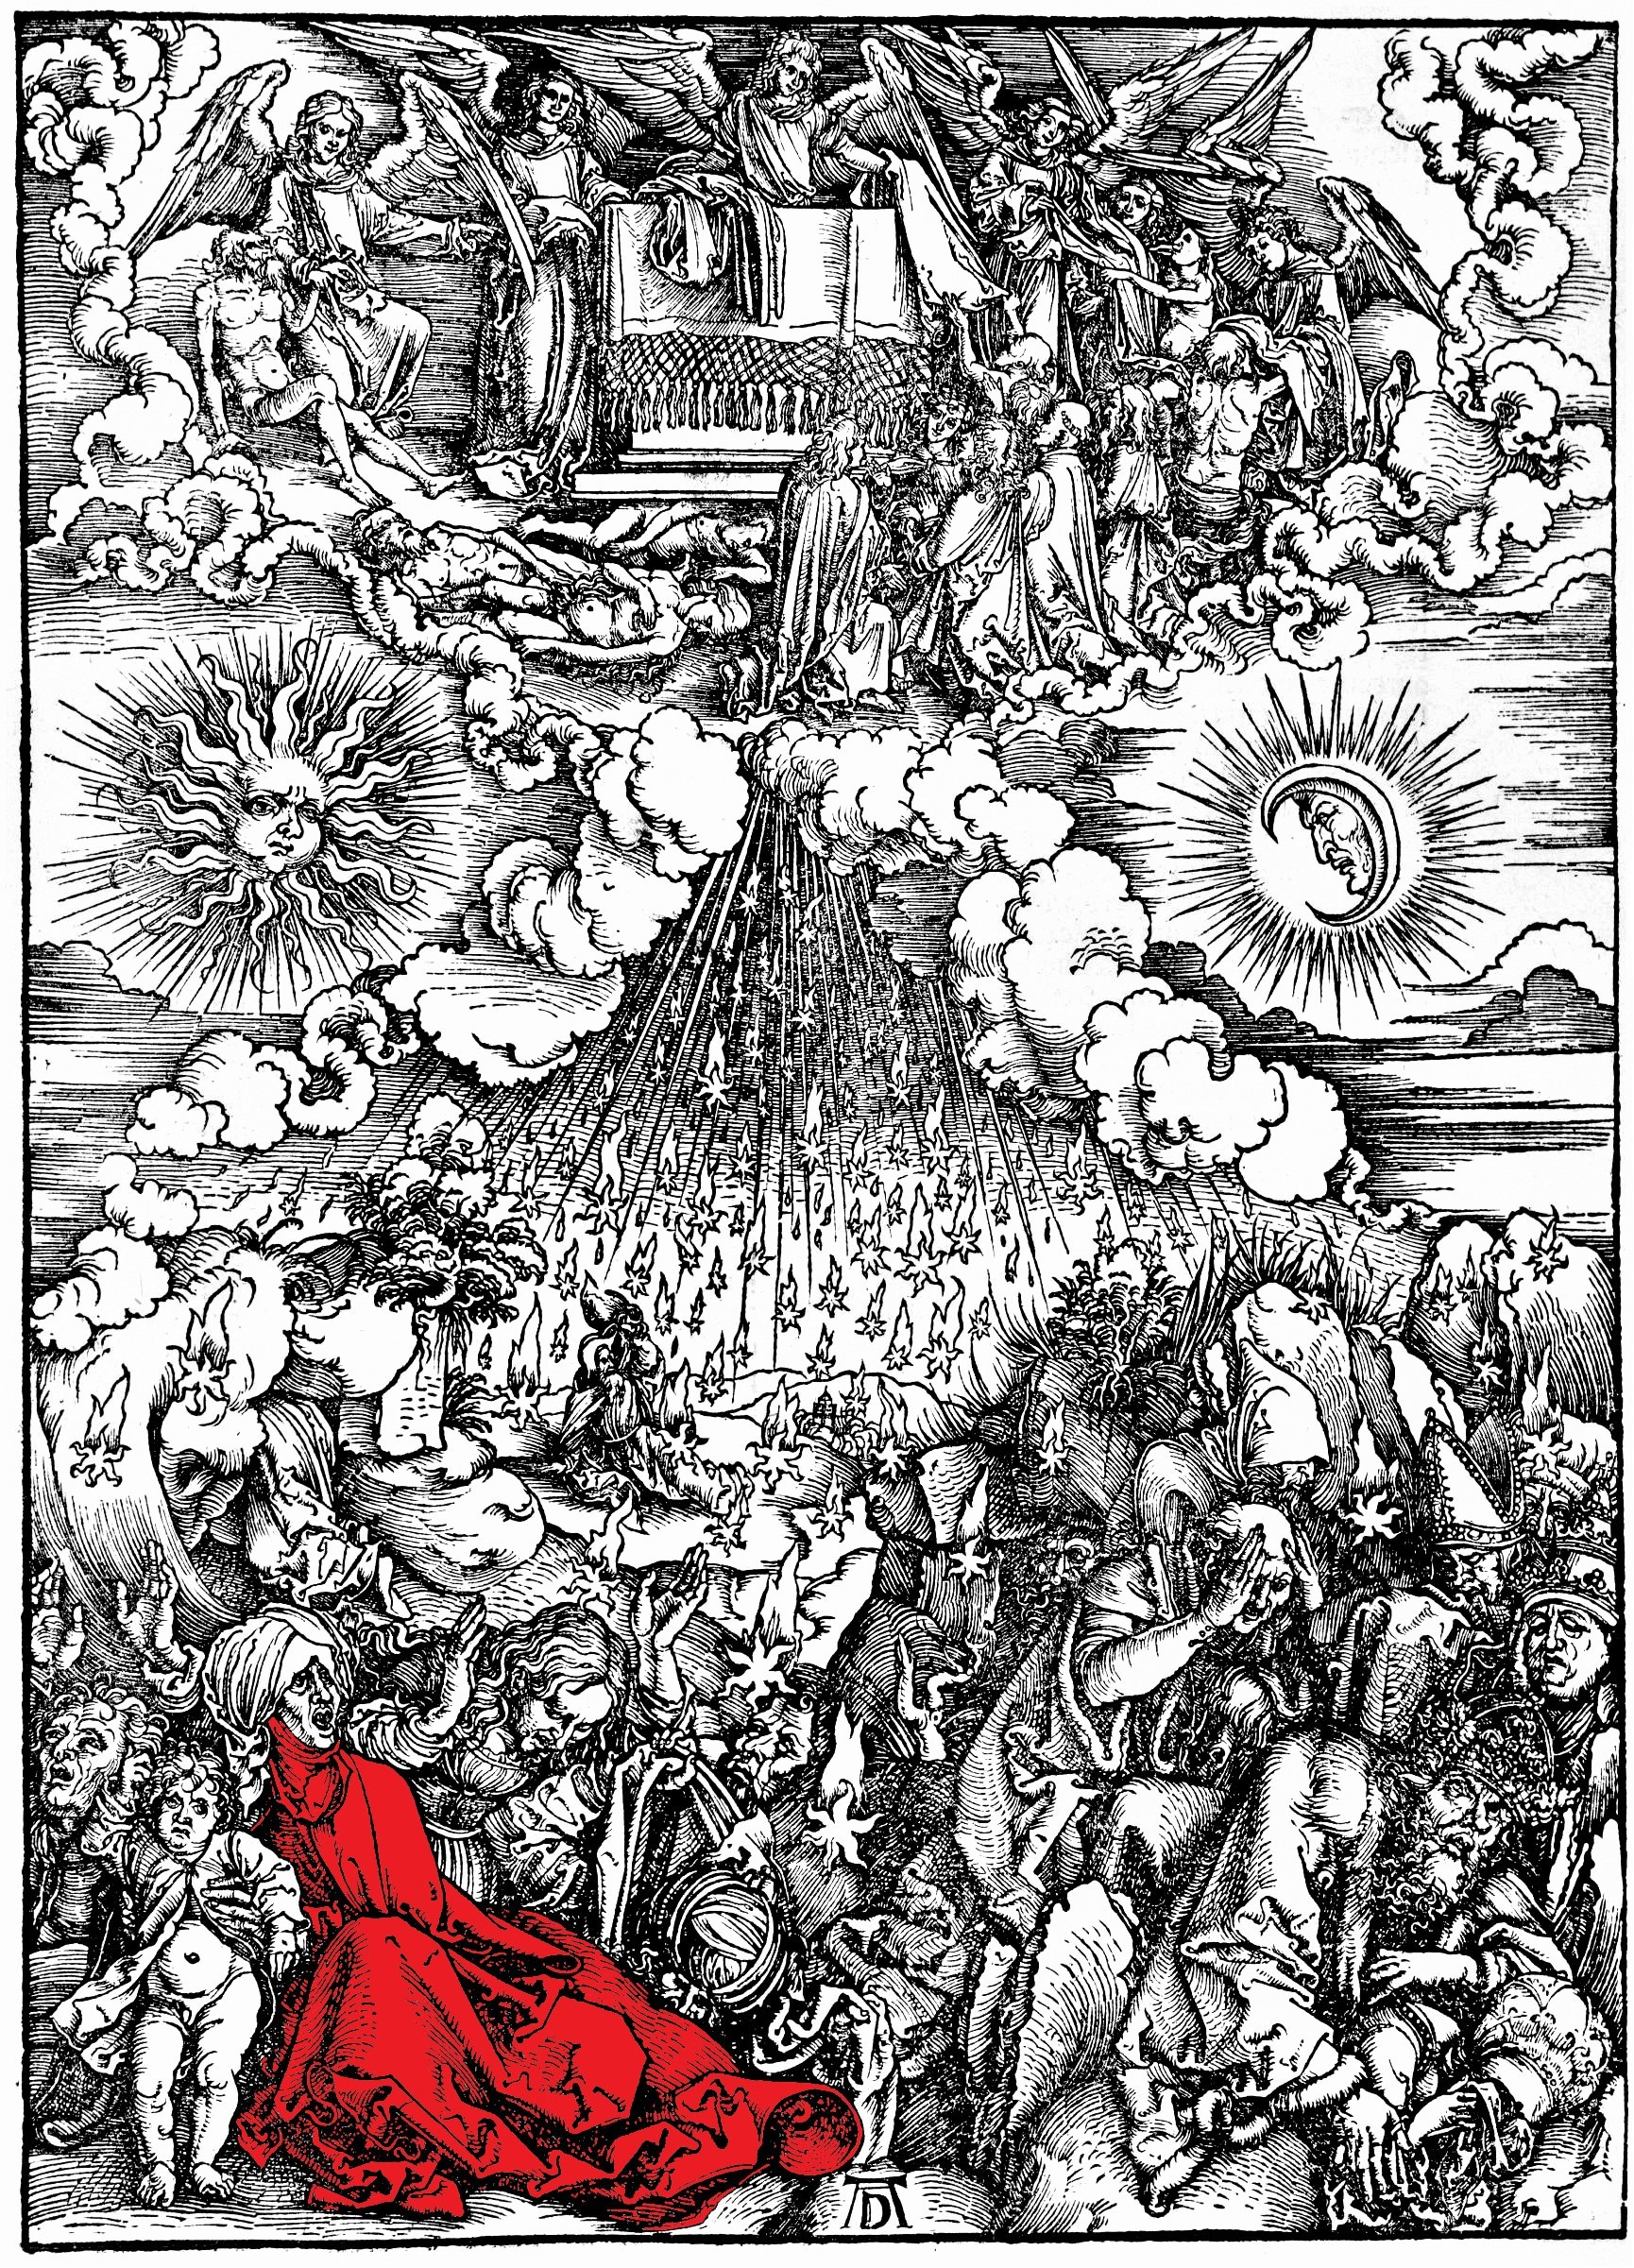
\includegraphics[width=\linewidth]{Durer/Durer_Sixth_Seal.jpg}
  	\caption[The Opening of the Fifth and Sixth Seals]{The Opening of the Fifth and Sixth Seals. Albrecht Dürer, 1498.}
  \end{figure*}
